\chapter{Gelijkvormigheid en uitwendige stroming}
\label{sec:Gelijkvormigheid en uitwendige stroming}
%%%%%%%%%%%%%%%%%%%%%%%%%%%%%%%%%%%%%%%%%%%%%%%%%%%%%%%%%%%%%%%%%%%%%%%%%%%%%%%%%%%%%%%%%%%%
\begin{toepassing}
	\label{oliepijplijn}
Olie met een viscositeit van 0.5\unit{Pa \cdot s} en een dichtheid van 830\unit{kg/m^3} wordt door een pijplijn met een diameter van 1m gepompt met een debiet van 1800\unit{m^3/h}. Er wordt een schaalmodel gebouwd dat gebruik maakt van buis met diameter 74mm en water ($\rho = 1000\unit{kg/m^3}$, $\nu = 1\unit{mm^2/s}$).

Bepaal de snelheid voor het model om gelijkvormigheid met betrekking tot viskeuze krachten te verkrijgen.

\end{toepassing}
\begin{antwoord}{\ref{oliepijplijn}}
	$v = 0.0143\unit{m/s}$
\end{antwoord}
\begin{toepassing}[*]
	\label{weerballon}
De ontwerpers van een weerballon willen achterhalen wat de luchtweerstand van de ballon is bij de maximaal verwachte relatieve windsnelheid van 5 m/s bij standaard atmosfeercondities ($\rho = 1.225\unit{kg/m^3}$, $\mu = 1.83\times 10^{-5}\unit{Pa \cdot s}$).
Hiervoor wil men een 1:20 schaalmodel testen in water bij 20\degC\ ($\rho = 998\unit{kg/m^3}$, $\mu = 1\times 10^{-3}\unit{Pa \cdot s}$). 
		
Bij welke watersnelheid moet men de tests uitvoeren opdat de data een voorspelling kunnen leveren van het gedrag van de balon in lucht? 
		
Als er een dragkracht van 2\unit{kN} wordt opgemeten bij deze snelheid, wat is dan de verwachte weerstandskracht bij het prototype?
\end{toepassing}
\begin{antwoord}{\ref{weerballon}}
	$v = 6.71\unit{m/s}$, $F = 0.55\unit{kN}$
\end{antwoord}
%%%%%%%%%%%%%%%%%%%%%%%%%%%%%%%%%%%%%%%%%%%%%%%%%%%%%%%%%%%%%%%%%%%%%%%%%%%%%%%%%%%%%%%%%%%%
\begin{toepassing}[*]
	\label{insect}
Het aerodynamisch gedrag van een vliegend insect wordt bestudeerd in een windtunnel met een 10:1 schaalmodel. In werkelijkheid klappert het insect 50 maal per seconde met de vleugels en vliegt het met een snelheid van \unit{1.25}{m/s} ten opzichte van de lucht. 
		
Kan volledige gelijkvormigheid behaald worden?
		
Bepaal de snelheid in de windtunnel en de klapfrequentie van het schaalmodel opdat de uitgevoerde metingen representatief zouden zijn voor de werkelijkheid.
\end{toepassing}
\begin{antwoord}{\ref{insect}}
	$v = 0.125\unit{m/s}$, $f = 0.5\unit{Hz}$
\end{antwoord}
%%%%%%%%%%%%%%%%%%%%%%%%%%%%%%%%%%%%%%%%%%%%%%%%%%%%%%%%%%%%%%%%%%%%%%%%%%%%%%%%%%%%%%%%%%%%
\begin{toepassing}[*]
	\label{onderzeeer}	
Een onderzeeër moet tegen een snelheid van 10 knopen (1 knoop = 0,5144 m/s) onder zeewater ($\rho = 1028\unit{kg/m^3}$, $\nu = 1.83\unit{mm^2/s}$) kunnen varen. Er wordt een experiment gedaan op schaal 1:20 in zoetwater ($\rho = 998\unit{kg/m^3}$, $\nu = 1.00\unit{mm^2/s}$).
		
Bepaal de snelheid waarop het model getest moet worden.
		
Bepaal het vermogen dat de onderzeeër voor voortstuwing nodig heeft als op het model een kracht van 200\unit{kN} wordt gemeten.
\end{toepassing}
\begin{antwoord}{\ref{onderzeeer}}
	$v = 56.2\unit{m/s}$, $P = 3549\unit{kW}$
\end{antwoord}
%%%%%%%%%%%%%%%%%%%%%%%%%%%%%%%%%%%%%%%%%%%%%%%%%%%%%%%%%%%%%%%%%%%%%%%%%%%%%%%%%%%%%%%%%%%%
\begin{toepassing}[*]
	\label{schip}
Een schip van 152.4\unit{m} lang vaart met een snelheid van 15 knopen (1 knoop = 0,5144m/s). Een model op schaal 1:25 wordt getest in hetzelfde water.

Bepaal de snelheid van het model voor :
	\begin{enumerate}
		\item Dynamische gelijkvormigheid voor oppervlaktegolven.
		\item Dynamische gelijkvormigheid voor wrijving.
	\end{enumerate}
\end{toepassing}
\begin{antwoord}{\ref{schip}}
	$v_{\text{oppervlaktegolven}} = 1.54\unit{m/s}$, $v_{\text{wrijving}} = 192.9\unit{m/s}$
\end{antwoord}
%%%%%%%%%%%%%%%%%%%%%%%%%%%%%%%%%%%%%%%%%%%%%%%%%%%%%%%%%%%%%%%%%%%%%%%%%%%%%%%%%%%%%%%%%%%%
\begin{toepassing}
	\label{spandoek}
Een vrij hangend spandoek opgespannen aan 2 lantaarnpalen kan onder bepaalde condities beginnen oscileren onder invloed van de wind. De oscilatie frequentie $f$ afhankelijk is van de breedte $b$ en hoogte $h$ van het spandoek, de windsnelheid $v$, de luchtdischtheid $\rho$ en de veerconstante $k$ van de ophanging.

Bepaal geschikte dimensieloze parameters om de dimensieloze frequentie uit te drukken. 

	\centering
	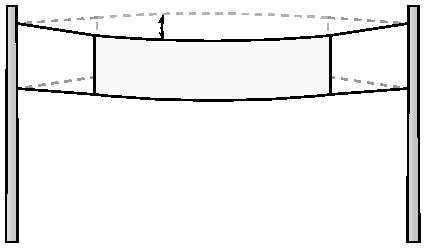
\includegraphics[width=0.48\textwidth]{fig/gelijkvormigheid/spandoek.pdf}
\end{toepassing}
\begin{antwoord}{\ref{spandoek}}
	$\frac{f}{vb} = \phi\left( \frac{h}{b},\frac{k}{\rho v^2 b} \right)$
\end{antwoord}
%%%%%%%%%%%%%%%%%%%%%%%%%%%%%%%%%%%%%%%%%%%%%%%%%%%%%%%%%%%%%%%%%%%%%%%%%%%%%%%%%%%%%%%%%%%%
\begin{toepassing}
	\label{vernauwing dimensieloos}
Bij een plotse vernauwing in een buis waarin een vloeistof stroomt is de drukval $\Delta p$ over de vernauwing afhankelijk van de dichtheid $\rho$ en de viscositeit $\mu$ van de vloeistof, de diameter voor $d_1$ en na $d_2$ en de snelheid voor de vernauwing $v$.

Bepaal geschikte dimensieloze parameters om de dimensieloze drukval uit te drukken. 
\end{toepassing}
\begin{antwoord}{\ref{vernauwing dimensieloos}}
	$\frac{\Delta p}{\rho v^2} = \phi\left( \frac{d_1}{d_2},\frac{\rho v d_1}{\mu} \right)$
\end{antwoord}